% Created 2024-02-23 周五 21:41
% Intended LaTeX compiler: xelatex
\documentclass[11pt]{article}
\usepackage{graphicx}
\usepackage{longtable}
\usepackage{wrapfig}
\usepackage{rotating}
\usepackage[normalem]{ulem}
\usepackage{amsmath}
\usepackage{amssymb}
\usepackage{capt-of}
\usepackage{hyperref}
\usepackage{ctex}
\usepackage[a4paper]{geometry}
\date{}
\title{Hamiltonian Operator Inference: Physics-preserving Learning of Reduced-order Models for Canonical Hamiltonian Systems}
\hypersetup{
 pdfauthor={},
 pdftitle={Hamiltonian Operator Inference: Physics-preserving Learning of Reduced-order Models for Canonical Hamiltonian Systems},
 pdfkeywords={},
 pdfsubject={},
 pdfcreator={Emacs 28.2 (Org mode 9.7-pre)}, 
 pdflang={English}}
\begin{document}

\maketitle
\section{Hamiltonian Operator Inference: Physics-preserving Learning of Reduced-order Models for Canonical Hamiltonian Systems}
\label{sec:org75a397e}
\subsection{Shortcoming of others}
\label{sec:org6b30608}
\begin{itemize}
\item 传统基于投影的侵入式降价算法是利用辛Galerkin方法将方程从全空间降维至辛子空间.这样的投影方法需要知道算子的全部信息并且可以控制代码的编写.
\item 标准的算子推断框架会破坏canonical Hamiltonian系统的物理结构.
\item 本文导出的Hamiltonian算子推断是在标准算子推断的基础之上嵌入了物理信息部分,从而保证不破坏物理系统的物理结构.
\end{itemize}
\subsection{Background}
\label{sec:orgb44ecf0}
\subsubsection{Hamiltonian System}
\label{sec:orgd9a34ce}
我们考虑无限维 Hamiltonian 系统,
\begin{equation}
\label{eq:1}
\frac{\partial y(x,t)}{\partial t}=\mathcal{S} \frac{\delta \mathcal{H}}{\delta y},
\end{equation}
其中 \(\mathcal{S}\) 是一个skew-symmetric算子(在Hilbert空间中,其满足 \(\mathcal{S}\subset-\mathcal{S}^{\star}\)),\(\frac{\delta \mathcal{H}}{\delta y}\) 表示 \(\mathcal{H}\) 的一阶变分导数.

我们定义Hamiltonian泛函 \(\mathcal{H}\) 为
\begin{equation}
\label{eq-Hamiltonianfunctional}
\mathcal{H}[y]=\int(H_{quad}(y,y_x,\cdots)+H_{nl}(y))\mathrm{d}x,
\end{equation}
其中 \(H_{quad}(y,y_x,\cdots)\) 表示二次项,其在变分过程中会导出线性项, \(H_{nl}(y)\) 表示Hamiltonian泛函中的非线性部分,其在变分过程中导出非线性部分.

为了保Hamiltonian系统的几何性质, 相关的数值模拟分为两步进行:
\begin{enumerate}
\item 使用保结构空间离散方法,降阶到一系列Hamiltonian ODEs.
\item 在上面的基础上, 对时间方向做保结构时间离散.
\end{enumerate}
\subsubsection{Space Discretization}
\label{sec:orgb07dad8}
我们利用离散化时空连续的Hamiltonian泛函 \eqref{eq-Hamiltonianfunctional} 来导出FOM. 我们给出最终的离散结果如下所示,
\begin{equation}
\label{space discretize FOM}
\dot{y}=S_d\nabla_yH_d(y)
\end{equation}
其中 \(S_d=-S_d^T\),其在离散层面上展示了 \(S\) 的反称性, \(H_d\) 表示空间离散的Hamiltonian泛函.

由于我们仅考虑canonical Hamiltonian系统,因此我们可以直接给出离散反称算子的结构为 \(S_d=J_{2n}=\begin{pmatrix}0&I_n\\-I_n&0\end{pmatrix}\). 此外,依据离散反称算子 \(S_d\) 的结构,我们可以将状态向量 \(y\in \mathbb{R}^{2n}\) 改写成 \(y=\begin{bmatrix}q^T,p^T\end{bmatrix}^T\).故而,我们可以将空间半离散canonical Hamiltonian系统改写为:
\begin{equation}
\dot{y}=\begin{bmatrix}\dot{q}\\ \dot{p}\end{bmatrix}=J_{2n}\nabla_y H_d(q,p)=\begin{bmatrix}\nabla_pH_d(q,p)\\-\nabla_qH_d(q,p)\end{bmatrix}
\end{equation}
根据我们导出的新形式来看,我们可以认为canonical Hamiltonian系统是一个耦合系统.事实上,我们划分的 \(q\) 和 \(p\) 分别具有对应的物理解释并且正是上述耦合的关系导致了canonical Hamiltonian系统具有对应的canonical辛结构.

我们给出一个例子来表示上述的划分是存在且有意义的.我们考虑描述一维简谐振动的波动方程,
\begin{equation*}
\frac{\partial^2u}{\partial t^2}=c^2 \frac{\partial^2u}{\partial x^2}
\end{equation*}
由于我们不考虑外加源项,因此我们可以得到物理系统的总能量为 \(E=\int_{\Omega}\frac{1}{2}u_t^2+\frac{1}{2}c^2u_x^2\mathrm{d}x\).我们假设该物理系统对应的广义坐标为 \(q=u\), \(q=u_t\),那么该系统的Hamiltonian为 \(\mathcal{H}=\int_{\Omega}\frac{1}{2}p^2+\frac{1}{2}c^2q_x^2\mathrm{d}x\).根据前面推出的canonical Hamiltonian系统的形式,我们可以得到如下的Hamiltonian系统,
\begin{align*}
&\dot{q}=\frac{\delta \mathcal{H}}{\delta p}=p\\
&\dot{p}=-\frac{\delta \mathcal{H}}{\delta q}=c^2q_{xx}
\end{align*}
如果我们考虑强迫振动的情况,也就是考虑外加源项 \(H_{nl}\) 的影响,无非只是在总能量中加入由外加源项提供的外加势能.
\subsubsection{Intrusive Structure-preserving Model Reduction}
\label{sec:orgddfc82a}
基于投影的模型降阶方法的主要做法是将半离散系统投影到低维子空间.在投影过程中最为关键的部分在于需要保持底层特征不变.由于前面构造的FOM是有辛结构的Hamiltonian系统,因此我们用低维子空间的辛提升的逆操作来进行投影.

辛子空间的辛提升定义为 \(y=V\tilde{y}\) ,其中 \(V\in\mathbb{R}^{2n\times2r}\) 是辛矩阵(其满足 \(V^TJ_{2n}V=J_{2r}\)), \(y\in \mathbb{R}^{2n}\) 是状态空间向量, \(\tilde{y}\in \mathbb{R}^{2n}\) 是低维子空间向量.辛矩阵 \(V\) 的辛逆矩阵 \(V^+\) 定义为 \(V^+=J_{2r}^TV^TJ_{2n}\).从其形式来看,我们可以进一步给出相关的性质, \(V^+\) 是 \(2r\times2n\) 维矩阵且其为 \(V\) 的左逆矩阵,
\begin{equation*}
V^TJ_{2n}V=J_{2r}\Rightarrow J_{2r}^TV^TJ_{2n}V=I_{2r}=V^+V
\end{equation*}
那么辛投影就可以被写作 \(\tilde{y}=V^+y\).辛投影后的降维状态向量对时间的求导满足,
\begin{equation*}
\dot{\tilde{y}}=V^+\dot{y}=V^+J_{2n}\nabla_yH_d(y)=J_{2r}V^T\nabla_yH_d(y)=J_{2r}\nabla_{\tilde{y}}H_d(V\tilde{y})
\end{equation*}
其中推导过程用到如下两条式子,
\begin{align*}
&V^+J_{2n}=J_{2r}^TV^T(-I_{2n})=-J_{2r}^TV^T=J_{2r}V^T\\
&\nabla_{\tilde{y}}H_d(y)=\nabla_{\tilde{y}}H_d(V\tilde{y})=\nabla_yH_d(V\tilde{y})\cdot \frac{\partial y}{\partial \tilde{y}}=V^T\nabla_yH_d(y)
\end{align*}
如此一来,我们就可以将得到一个 \(2r\) 维的ROM,
\begin{equation*}
\dot{\tilde{y}}=J_{2r}\nabla_{\tilde{y}}\tilde{H}(\tilde{y})
\end{equation*}
其中 \(\tilde{y}\) 是降维状态向量, \(\tilde{H}(\tilde{y})=H_d(V\tilde{y})\) 则是
降维的Hamiltonian.显然, \(\tilde{H}\) 的导出依托于对 \(H_d\) 的结构已知.

上述推导中关键在于如何选取辛投影矩阵 \(V\).Proper symplectic decomposition(PSD)是选取辛投影矩阵的一种方法,其主要含义是找一个合适的辛矩阵 \(V\) 来最小化投影误差,
\begin{equation*}
\min_V \left\Vert Y-VV^+Y\right\Vert_F
\end{equation*}
其中 \(Y=\begin{bmatrix}y(t_1),\cdots,y(t_K)\end{bmatrix}\in\mathbb{R}^{2n\times K}\) 是快照数据矩阵.如果在全局寻找最优的辛矩阵,其需要较大的计算量,下面给出三个寻找次优解的优化策略(不同的优化策略本质上是在不同的子空间中寻找次优解)

\begin{center}
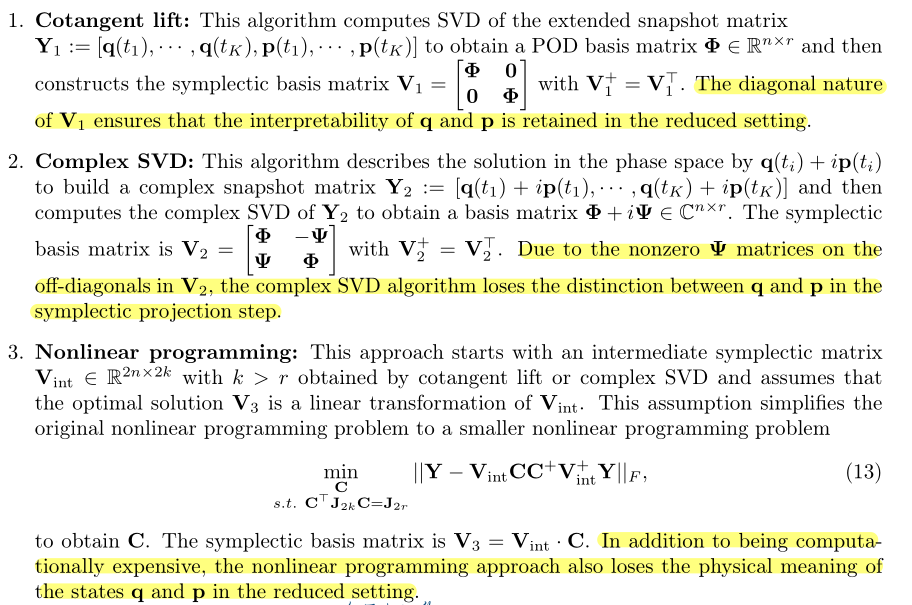
\includegraphics[width=.9\linewidth]{img/Background/2024-02-23_00-00-58_screenshot.png}
\end{center}

上述三种优化方法的严谨讨论在\href{PM2015SymplecticModelReduction.org}{Symplectic Model Reduction of Hamiltonian Systems}介绍.
\subsection{Standard Operator Inference}
\label{sec:orgeb006c4}
针对一维简谐振动方程,我们推导相应的FOM,
\begin{equation*}
\dot{y}=J_{2n}\nabla_yH_d(y)=\begin{bmatrix}0&I_n\\-I_n&0\end{bmatrix}\begin{bmatrix}-c^2D_{fd}&0\\0&I_n\end{bmatrix}y=\begin{bmatrix}0&I_n\\c^2D_{fd}&0\end{bmatrix}y
\end{equation*}
其中的 \(D_{fd}\) 表示对二阶求导算子的有限差分逼近矩阵.至于获取快照数据矩阵的方法无非是在此FOM的基础上对时间方向进行离散求解得到的数据组合而成.

我们用此线性波动方程为例来验证标准的算子推断会破坏系统的物理结构从而导出数值不稳定的降阶模型.首先,我们需要对快照数据矩阵 \(Y\) 进行SVD得到相应的Proper Orthogonal Decomposition(POD)基矩阵 \(V\), 其中 \(V\) 的列向量是POD的基向量,
\begin{equation*}
V=\begin{bmatrix}v_1,\cdots,v_{2r}\end{bmatrix}\in \mathbb{R}^{2n\times2r}
\end{equation*}
\end{document}